\documentclass[../../thesis.tex]{subfiles}

\begin{document}


\section{Implementation details}

In our implementation, we closely follow to the methodology outlined in \cite{TimeVQVAE}, particularly in the design and deployment of the encoder, decoder, and codebook.

\subsubsection{Time Frequency Modelling}
We utilize the Short Time Fourier Transform (STFT) and its inverse (ISTFT) for time-frequency modeling, employing \texttt{torch.stft} and \texttt{torch.istft} functions, respectively. Consistent with \cite{TimeVQVAE}, we set the primary parameter \texttt{nfft} to 8 and maintain default settings for others. This configuration yields a frequency axis spanning $[1, 2, 3, 4, 5]$ and a time axis half the length of the original.

\subsubsection{Encoder and decoder}

The encoder and decoder architectures closely resemble those described in \cite{nadavbh12}, with further adaptations from \cite{TimeVQVAE}.\newline

As illustrated in Figure \ref{fig:VQVAE Encoder}, the encoder consists of $n$ downsampling convolutional blocks (\texttt{Conv2d - BatchNorm2d - LeakyReLU}), followed by $m$ residual blocks (\texttt{LeakyReLU - Conv2d - BatchNorm2d - LeakyReLU - Conv2d}). Downsampling convolutional layers are implemented with parameters: \texttt{kernel size=(3,4), stride=(1,2), padding=(1,1)}, downsampling the temporal axis by a factor of 2 per block. Residual convolutional layers have parameters: \texttt{kernel size=(3,3),stride=(1,1), padding=(1,1)}. The decoder mirrors this architecture, featuring $m$ residual and $n$ upsampling layers using transposed convolutional blocks with identical parameters.\newline

The downsampling rate is determined by $2^n$, ensuring the resulting latent representation ($z$) has a width of 32. For a comprehensive understanding of the TimeVQVAE implementation details, we direct readers to Appendix C.3 of \cite{TimeVQVAE}.

\begin{figure}[h]
    
    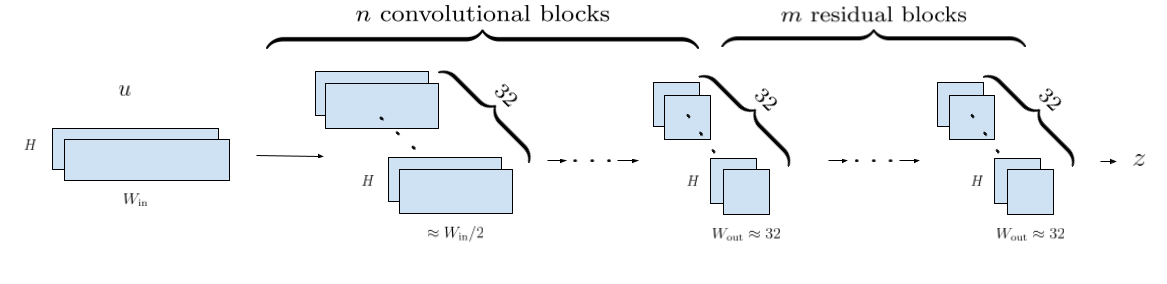
\includegraphics[scale = 0.30]{VQVAE Encoder.png}
    \centering
    \caption{Overview of the encoder architecture. The decoder architecture is simply obtained by reversing the arrows and switching out the convolutional block for transposed convolutional blocks.}
    \label{fig:VQVAE Encoder}
\end{figure}

\subsubsection{VQ}
% Implementation from lucidrains/vector-quantize-pytorch.
%  https://github.com/lucidrains/vector-quantize-pytorch \newline
We adopt a codebook size of 32 and a dimension of 64, utilizing exponential moving average with a decay of 0.9 and a commitment loss with weight $\beta = 1$.

\subsubsection{Augmentations}
window warp:    window ratio: 0.4,min window warp: 0.9, max windowwarp: 2.0\newline
amplitude resize: Amp Rrate: 0.2\newline
gaussian noise: gaus mean: 0, gaus std: 0.05\newline
slice and shuffle:

\subsubsection{SSL}
For both Barlow Twins and VIbCReg, we implement the projector following the guidelines in \cite{lee2024computer}. The projector's dimension size is set to 4096 for both methods, with $\lambda$ set to $5 \times 10^3$ for Barlow Twins. For VIbCReg, $\lambda$ and $\mu$ are both set to 25, while $\nu$ is set to 100.

\subsubsection{Prior learning}
In the iterative decoding algorithm, the number of iterations $T$ is set to 10, following \cite{chang2022maskgit}. We employ cosine as the mask scheduling function ($\gamma$), adopting the implementation from \cite{TimeVQVAE}. 


\subsubsection{Optimizer}
We utilize the AdamW optimizer with batch sizes set to 128 for stage 1 and 256 for stage 2, an initial learning rate of $10^{-3}$, cosine learning rate scheduler, and a weight decay of $10^{-5}$. Both stage 1 and stage 2 training procedures run for 1000 epochs.
\subsubsection{Evaluation}
For downstream classification, K-nearest neighbors (KNN) and Support Vector Machines (SVM) are implemented using scikit-learn, with $K=5$ for KNN and a linear kernel for SVM. 
% Additionally, SupervisedFCN \cite{VQVAE} is employed for calculating Inception Score (IS), Fréchet Inception Distance (FID), and Consistency Accuracy Score (CAS).

\section{Initial Experimentation and Model Development}

The overarching objective in creating our model is to learn more expressive latent representations for better time series generation. We want to keep the reconstruction capabilities of the tokenization model at a high level, where the rationality is that if the tokenization model reconstructs well the latent representations contains all relevant information of the input. We simultaneously want enforce better class separability in the latent representations, as we hypothesize that such additional structure eases/improved learning of the generative model.\newline

During development we encountered several problems:\newline
When we attempted a siamese architecture, with quantization in the augmented branch, and to derive the SSL loss from the discrete representations there were a correlation problem. The codewords were very highly correlated, which resulted from the passing both views through the VQ.  $SSL(z_q,z_q')$ \newline
In an attempt to solve this we attempted to derive the SSL loss from the continuous latent representations, but the resulting discrete latent representations performed poorly on the downstream classification task. Separability problem: $SSL(z,z')$ \newline
The solution was to remove the VQ in the augmented branch and rather derive the SSL loss from $z_q$ and $z'$. Solution: $SSL(z_q,z')$ \newline

Overfitting problem: Using $SG()$ on augmented branch / Not using augRecons \newline

\section{Main Experiments}

In this thesis, we focus on two main objectives. Firstly, in Stage 1, we aim to determine whether NC-VQVAE can learn more expressive representations compared to VQVAE. Specifically, we investigate whether NC-VQVAE can achieve reconstruction performance on par with VQVAE while simultaneously enhancing downstream classification. In Stage 2, our interest lies in examining the impact of NC-VQVAE on prior learning and time series generation.\newline

To evaluate our model, NC-VQVAE, we compare it against the naive VQVAE using both Barlow Twins and VIbCReg as self-supervised learning (SSL) methods. For each SSL method, we train three distinct models employing different sets of augmentations. Furthermore, each configuration is trained using four different seeds, resulting in a total of 364 models trained at each stage.\newline

Our evaluation process begins with assessing the tokenization models, focusing on their reconstruction capability and performance in downstream classification tasks. Subsequently, we proceed to train a prior model on top of the various tokenization models. We then evaluate the performance of the generative models using metrics such as IS (Inception Score), FID (Fréchet Inception Distance), and CAS (Classification Accuracy Score). Additionally, visual inspections are conducted at both stages to provide further insights into the models' performance.\newline


\section{Stage 1}
\TODO{hyperparameters}

One of the most interesting aspects of out model is the choice of augmentations. 

\subsection{Augmentations}
In our experiments we consider three sets of augmentations with different characteristics. They are
\begin{itemize}
    \item Amplitude Resizing + Window Warp
    \item Slice and Shuffle
    \item Gaussian noise
\end{itemize}

\textbf{Amplitude Resizing + Window Warp} scales in both x and y direction. The window warp has similar qualities to phase shift, but not uniformly and keeps endpoints fixed. They were considered as the observed conditional distribution in some datasets, such as ShapesAll \ref{fig:datasets}, had similar overall shape, but peaked with different amplitude and at different locations. Thus the augmented view had similar characteristics as the conditional distribution of the original view \ref{fig:ShapesAll_winwarp}. In many cases we will refer to this set of augmentations simply as warp. \newline

\begin{figure}[h]
    \centering
    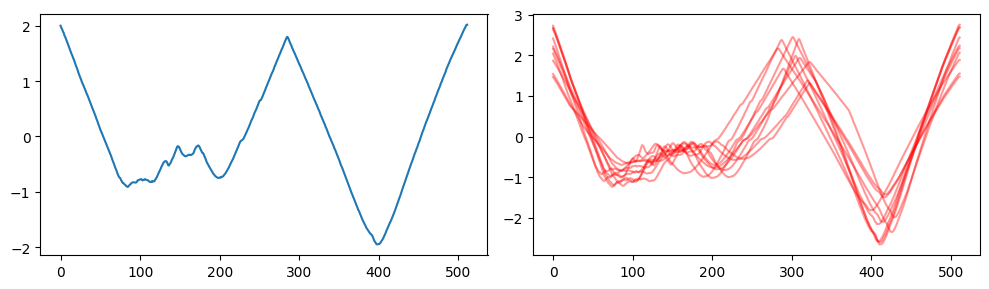
\includegraphics[scale = 0.3]{ShapesAll_winwarp.png}
    \caption{ShapesAll: Original (left), augmented (right). 15 instances of Amplitude Resizing + Window Warp applied to the original sample.}
    \label{fig:ShapesAll_winwarp}
\end{figure}

\textbf{Slice and Shuffle} crops the time series into four sections and permutes them. For datasets with sharp modularity and few peaks, such as ElectricDevices \ref{fig:datasets}, the augmentation provides a view with peaks occurring at timestamps not seen in the training data, which is illustrated in figure \ref{fig:ElectricDevices_SliceAndShuffel}. This could improve the reconstruction on unseen data, as well as encouraging the model to focus more on the existence of a peak rather than its specific location. For some datasets such as FordA \ref{fig:datasets}, the semantics of the dataset is preserved under this augmentation, despite their continuous nature. In many cases we will refer to this augmentation simply as slice.\newline
\begin{figure}[h]
    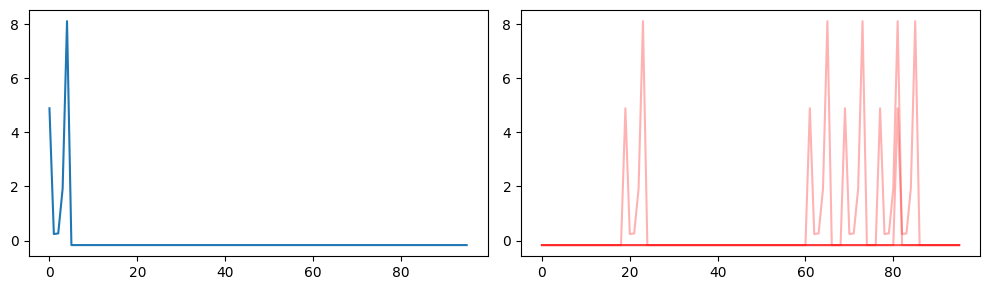
\includegraphics[scale = 0.3]{ElectricDevices_SliceAndShuffel.png}
    \centering
    \caption{ElectricDevices: Original (left), augmented (right). 5 instances of Slice and Shuffle applied to the original sample.}
    \label{fig:ElectricDevices_SliceAndShuffel}
\end{figure}


\textbf{Gaussian noise} adds a nose $\epsilon \sim N(0,0.05)$ to each datapoint in the time series. This introduces, in many cases, a substantial high frequency component as seen in figure \ref{fig:StarLight_Gaussian}. As the naive VQVAE described in \cite{TimeVQVAE} had trouble with reconstruction of HF components, this augmentation could provide more emphasis on these. The reconstruction of the augmented views can too provide more information regarding HF components for the decoder. Of the three augmentations, gaussian noise provides the most predictable augmented views from a numerical standpoint, which might result in a SSL loss which is easier to minimize. In many cases we will refer to this augmentation simply as Gaussian or gauss.

\begin{figure}[h]
    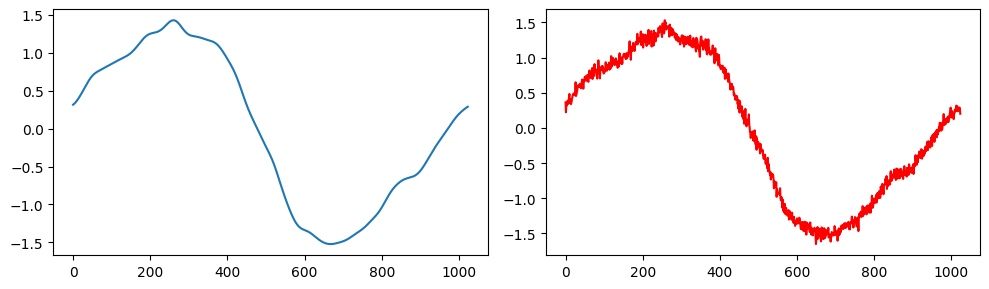
\includegraphics[scale = 0.3]{StarLight_Gaussian.png}
    \centering
    \caption{StarLightCurves: Original (left), augmented (right). One instance of Gaussian noise applied to the original sample.}
    \label{fig:StarLight_Gaussian}
\end{figure}

\subsection{Evaluation}

The tokenization model, as we are interested in representation learning, is evaluated on two metrics. Firstly, and most importantly its ability to reconstruct the input data once compressed into latent space. In essence the latent representation encodes "everything" (important information is preserved) about the original data if the model is able to reconstruct well. Secondly we evaluate linear classifiers on the latent representations, which provides good results if the model learns discriminative features of the different classes and produces an approximately linear separable space. Finally, as the tokenization model is a part of the generative model, the ultimate evaluation metric is the corresponding evaluation of the generative model. 



\section{Stage 2}

hyperparameters and details for stage 2.

\subsection{Evaluation}
How do we calculate the different metrics.


\begin{itemize}
    \item \textbf{IS}:
    \item \textbf{FID}:
    \item \textbf{CAS}:We evaluate the CAS for TSTR by using the Supervised FCN on all our models considered and compare against the baseline model to investigate the relative performance. 
    \item \textbf{Visual inspection}:
    \item \textbf{Token usage}:
\end{itemize}


\section{UCR Time Series Classification Archive}
The evaluation of our model NC-VQVAE is done on a subset of the UCR Time Series Archive \cite{UCRArchive2018}. The UCR archive is a collection of 128 datasets of univariate time series for time series classification. The different datasets in the archive span a wide range characteristics and include among others sensor, device, image-derived and simulated data. Each dataset has a predefined training and test split.\newline

Our subset of the UCR archive is presented in Table \ref{tab:UCRsubset.}

\begin{table}[h]
    \centering
    \begin{tabular}{llllll}
    \toprule
    Type      & Name                    & Train & Test & Class & Length \\
    \midrule
    Device    & ElectricDevices         & 8926  & 7711 & 7     & 96     \\
    Sensor    & FordB                   & 3636  & 810  & 2     & 500    \\
    Sensor    & FordA                   & 3601  & 1320 & 2     & 500    \\
    Sensor    & Wafer                   & 1000  & 6164 & 2     & 152    \\
    Simulated & TwoPatterns             & 1000  & 4000 & 4     & 128    \\
    Sensor    & StarLightCurves         & 1000  & 8236 & 3     & 1024   \\
    Motion    & UWaveGestureLibraryAll  & 896   & 3582 & 8     & 945    \\
    ECG       & ECG5000                 & 500   & 4500 & 5     & 140    \\
    Image     & ShapesAll               & 600   & 600  & 60    & 512    \\
    Simulated & Mallat	                & 55	& 2345 & 8	   & 1024   \\
    Image     & Symbols                 & 25    & 995  & 6     & 398    \\
    Sensor    & SonyAIBORobotSurface2   & 27    & 953  & 2     & 65     \\
    Sensor    & SonyAIBORobotSurface1   & 20    & 601  & 2     & 70     \\
    \bottomrule
    \end{tabular}
    \caption{The subset of the UCR Archive considered for our experiments.}
    \label{tab:UCRsubset}
    \end{table}

We choose to test on a subset, rather than on the entire UCR Archive, due to computational limitations as well as to more thoroughly investigate the effect of our models and the role of augmentations. The subset is chosen such that they span a wide range of train set sizes, lengths, classes and type, while the class distributions have visually different characteristics which can be seen from table \ref{tab:UCRsubset} and figure \ref{fig:datasets}. 

\begin{figure}[h]
    \centering
    \begin{minipage}[b]{0.32\textwidth}
        \centering
        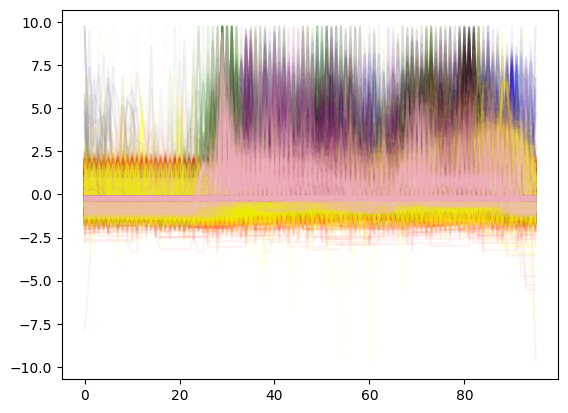
\includegraphics[width=\textwidth]{ElectricDevices}
        \caption*{ElectricDevices}
    \end{minipage}
    \hfill
    \begin{minipage}[b]{0.32\textwidth}
        \centering
        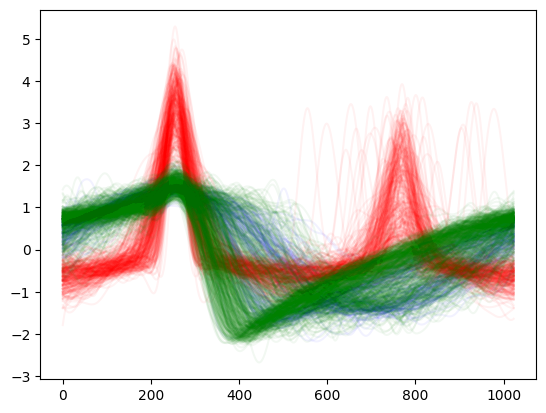
\includegraphics[width=\textwidth]{StarLightCurves}
        \caption*{StarLightCurves}
    \end{minipage}
    \hfill
    \begin{minipage}[b]{0.32\textwidth}
        \centering
        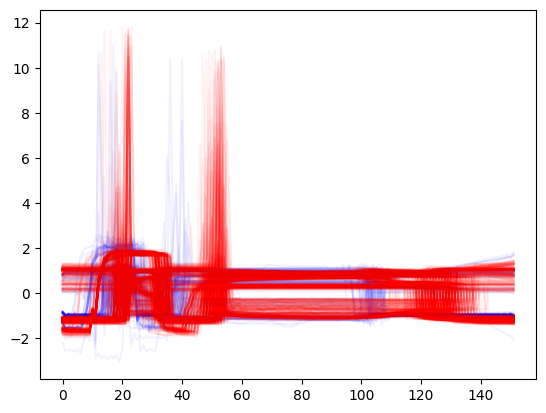
\includegraphics[width=\textwidth]{Wafer}
        \caption*{Wafer}
    \end{minipage}
    
    \vspace{0.4cm}
    
    \begin{minipage}[b]{0.32\textwidth}
        \centering
        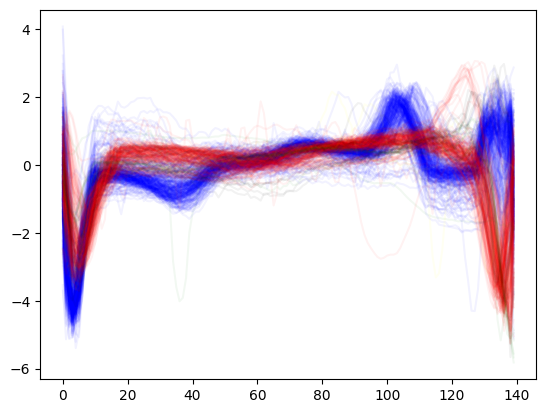
\includegraphics[width=\textwidth]{ECG5000}
        \caption*{ECG5000}
    \end{minipage}
    \hfill
    \begin{minipage}[b]{0.32\textwidth}
        \centering
        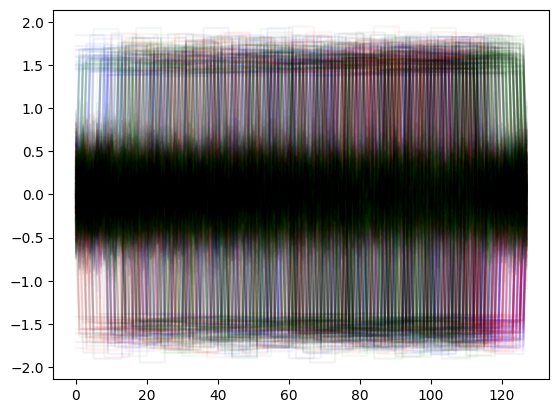
\includegraphics[width=\textwidth]{TwoPatterns}
        \caption*{TwoPatterns}
    \end{minipage}
    \hfill
    \begin{minipage}[b]{0.32\textwidth}
        \centering
        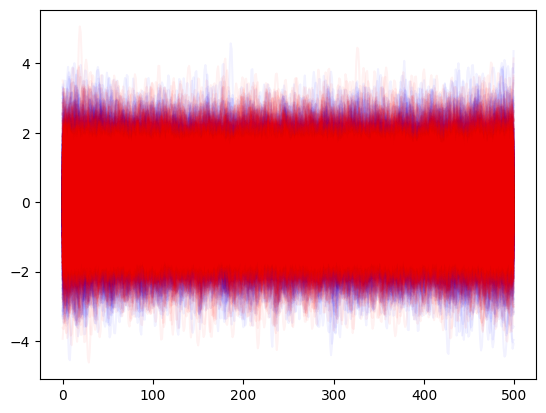
\includegraphics[width=\textwidth]{FordA}
        \caption*{FordA}
    \end{minipage}
    
    \vspace{0.4cm}
    
    \begin{minipage}[b]{0.32\textwidth}
        \centering
        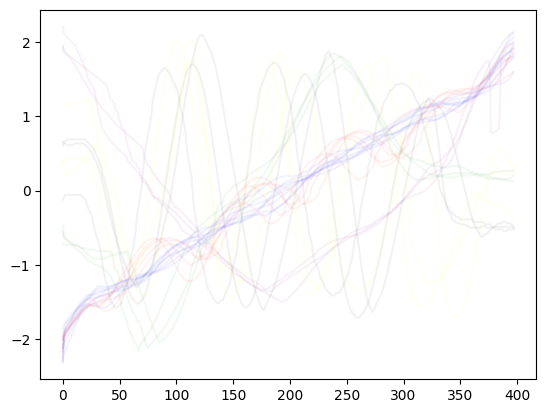
\includegraphics[width=\textwidth]{Symbols}
        \caption*{Symbols}
    \end{minipage}
    \hfill
    \begin{minipage}[b]{0.32\textwidth}
        \centering
        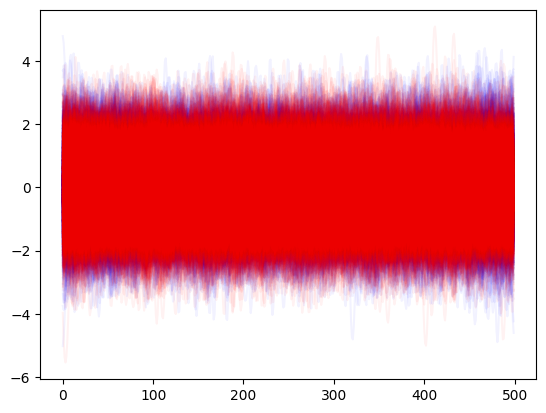
\includegraphics[width=\textwidth]{FordB}
        \caption*{FordB}
    \end{minipage}
    \hfill
    \begin{minipage}[b]{0.32\textwidth}
        \centering
        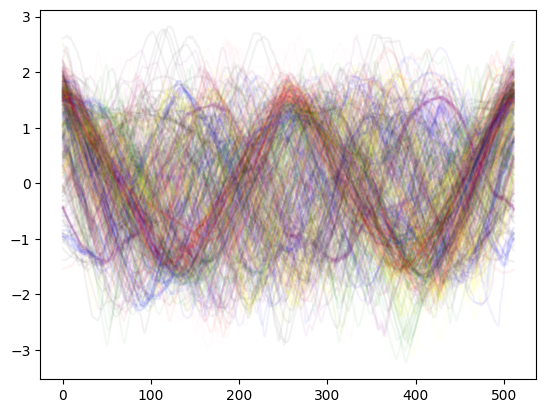
\includegraphics[width=\textwidth]{ShapesAll}
        \caption*{ShapesAll}
    \end{minipage}
    
    \vspace{0.4cm}
    
    \begin{minipage}[b]{0.32\textwidth}
        \centering
        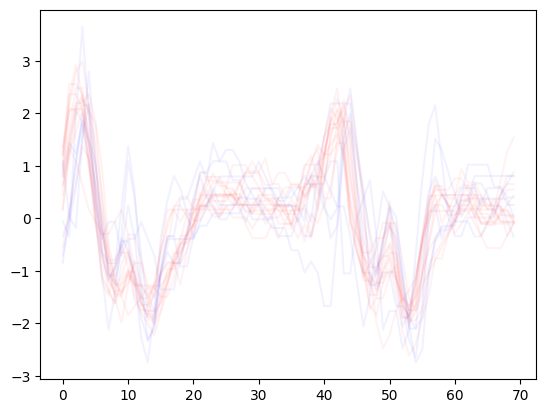
\includegraphics[width=\textwidth]{Sony1}
        \caption*{SonyAIBORobotSurface1}
    \end{minipage}
    \hfill
    \begin{minipage}[b]{0.32\textwidth}
        \centering
        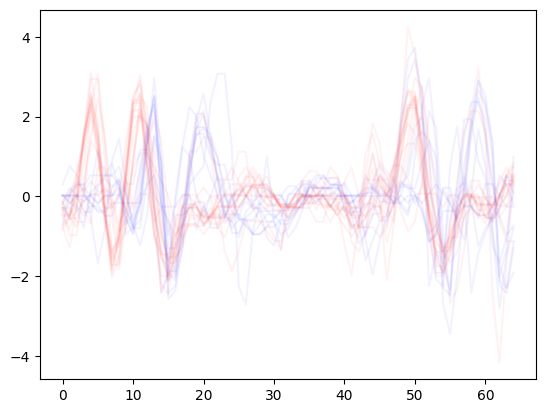
\includegraphics[width=\textwidth]{Sony2}
        \caption*{SonyAIBORobotSurface2}
    \end{minipage}
    \hfill
    \begin{minipage}[b]{0.32\textwidth}
        \centering
        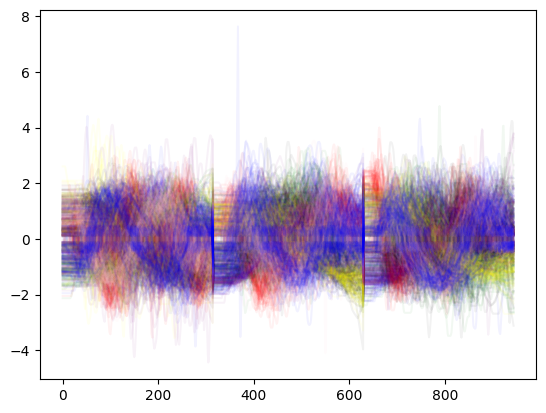
\includegraphics[width=\textwidth]{UWave}
        \caption*{UWaveGestureLibraryAll}
    \end{minipage}
    
    \vspace{0.4cm}
    
    \begin{minipage}[b]{0.32\textwidth}
        \centering
        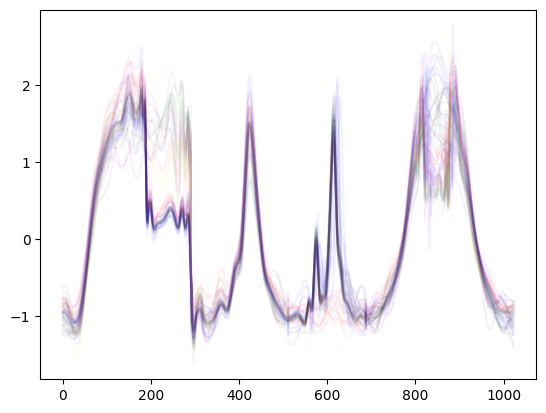
\includegraphics[width=\textwidth]{Mallat}
        \caption*{Mallat}
    \end{minipage}
    \caption{Our selected subset of the UCR Archive. All time series in the training set are plotted and color coded according to label.}
    \label{fig:datasets}
\end{figure}



\end{document}